% ---------------------------------------------------------------------------
% fig_gradient_utilisation.tex
% Gradient utilisation GU = 1 - ZVF against GRPO group size G.
%
% REAL DATA (all plotted numbers are measured, none invented):
%   platform_hybrid/experiments/results/groupsize_zvf_sweep.json
%     Qwen/Qwen2.5-0.5B, arithmetic_correctness, 40 steps, 16 prompts,
%     G in {2,4,8,16}, seeds {42,123,456} (n = 3 per G).
%     Per-G mean_zvf taken from .summary; SE recomputed from the three
%     per-seed mean_zvf values in .runs.
%       G=2  ZVF 0.8380 -> GU 0.1620 +/- 0.0073
%       G=4  ZVF 0.7635 -> GU 0.2365 +/- 0.0090
%       G=8  ZVF 0.6906 -> GU 0.3094 +/- 0.0068
%       G=16 ZVF 0.6312 -> GU 0.3688 +/- 0.0048
%   Power-law fit re-derived here from those four means:
%       log10(ZVF) = -0.0354 - 0.1371 log10(G)  =>  ZVF = 0.9217 G^-0.1371
%       R^2 = 0.99959  => GU(G) = 1 - 0.9217 G^-0.1371
%   Marginals cross-checked against
%   platform_hybrid/paper/sections/group_size.tex (the "falling marginal
%   benefit per doubling" paragraph, 0.075 vs 0.059) and
%   platform_hybrid/experiments/results/group_size_effect.tsv.
%
% CAVEATS HONOURED IN THE DRAWING:
%   * GU never approaches 1: at G=16 it is 0.369, i.e. 63% of groups are
%     still variance-dead. The figure does NOT draw a GU=1 ceiling or any
%     saturation asymptote near it -- the flattening shown is the falling
%     marginal return per doubling, not convergence onto full utilisation.
%   * The absolute per-doubling gains 0.074 / 0.073 / 0.059 fall only
%     slightly; the monotone decline is clearest in RELATIVE terms
%     (46% / 31% / 19% of the previous level). Panel (b) encodes both.
%   * G=32 is NOT a trained cell. It appears only as a dotted extrapolation.
%   * The repo string
%       group_size_effect.tsv :: zvf_loglog_slope
%         = "log10(mean_zvf) ~ 0.9042 + -0.2303*log10(G), R=-0.999"
%     is self-inconsistent (it predicts ZVF = 6.8 at G=2) and is NOT used.
%     The fit above was re-derived from the raw per-seed values.
%   * group_size_iter115_zvf_linkage.tsv reports "GU" > 1 (e.g. 2.42),
%     so those columns are not 1 - ZVF and are NOT used.
% ---------------------------------------------------------------------------
\documentclass[border=6pt]{standalone}
\usepackage{tikz}
\usepackage{pgfplots}
\pgfplotsset{compat=1.18}
\usetikzlibrary{arrows.meta,positioning,shapes.geometric,fit,backgrounds,calc,decorations.pathreplacing,patterns,pgfplots.groupplots}
\tikzset{
  blk/.style={rectangle, rounded corners=2pt, draw=black!70, thick, fill=blue!6,
              minimum height=8mm, minimum width=20mm, align=center, font=\small},
  io/.style={rectangle, rounded corners=6pt, draw=black!70, thick, fill=green!8,
             minimum height=8mm, align=center, font=\small},
  proc/.style={rectangle, draw=black!70, thick, fill=orange!10, minimum height=8mm,
               align=center, font=\small},
  dec/.style={diamond, aspect=2, draw=black!70, thick, fill=yellow!15, align=center, font=\footnotesize},
  warnbox/.style={rectangle, rounded corners=2pt, draw=red!60!black, thick, fill=red!7,
                  minimum height=8mm, align=center, font=\small},
  oklbox/.style={rectangle, rounded corners=2pt, draw=green!45!black, thick, fill=green!8,
                 minimum height=8mm, align=center, font=\small},
  ar/.style={-{Latex[length=2mm]}, thick},
  arl/.style={-{Latex[length=2mm]}, thick, dashed, draw=black!55},
  lbl/.style={font=\footnotesize\itshape, text=black!60},
}
\definecolor{good}{RGB}{34,139,34}
\definecolor{bad}{RGB}{178,34,34}
\definecolor{warn}{RGB}{218,165,32}
\definecolor{pesblue}{RGB}{0,45,98}
\definecolor{complete}{RGB}{30,125,79}
\definecolor{partial}{RGB}{176,106,0}
\definecolor{blocked}{RGB}{166,43,43}
% --- figure-local styles -------------------------------------------------
\pgfplotsset{
  myaxis/.style={
    width=7.3cm, height=5.7cm,
    tick label style={font=\scriptsize},
    label style={font=\footnotesize},
    title style={font=\footnotesize\bfseries, yshift=-1.5mm},
    legend style={font=\tiny, draw=black!30, fill=white, fill opacity=0.92,
                  text opacity=1, inner sep=2pt, row sep=1pt, cells={anchor=west}},
    grid=major, grid style={draw=black!12},
    axis line style={draw=black!60},
    tick align=outside,
  }
}
\begin{document}
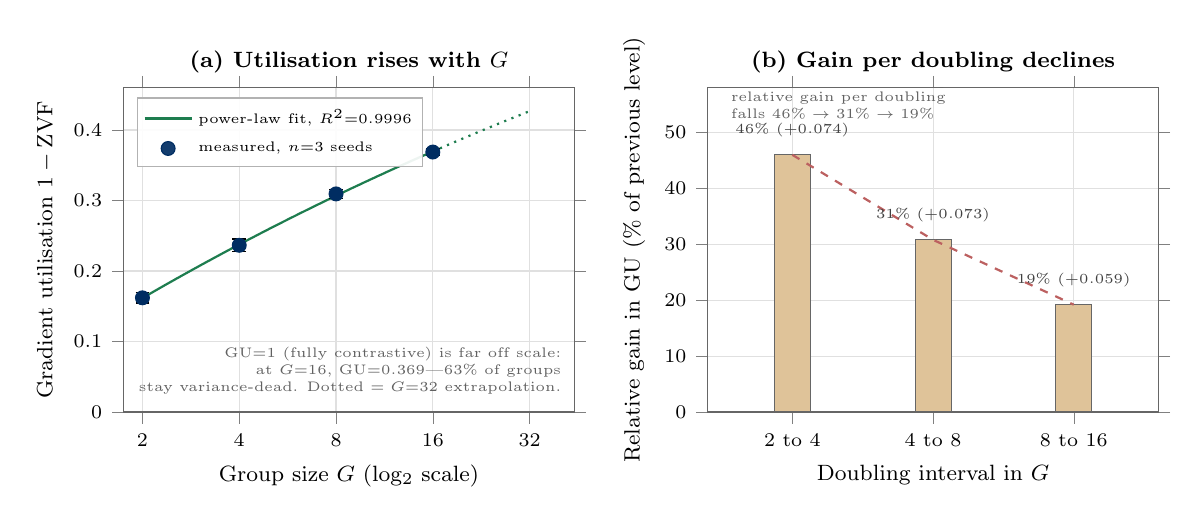
\begin{tikzpicture}
\begin{groupplot}[
  group style={group size=2 by 1, horizontal sep=1.7cm, ylabels at=edge left},
  myaxis
]

% ================== (a) gradient utilisation vs G =======================
\nextgroupplot[
  title={(a) Utilisation rises with $G$},
  xlabel={Group size $G$ (log$_2$ scale)},
  ylabel={Gradient utilisation $1-\mathrm{ZVF}$},
  xmode=log, log basis x=2,
  xtick={2,4,8,16,32}, xticklabels={2,4,8,16,32},
  xmin=1.75, xmax=44,
  ymin=0, ymax=0.46, ytick={0,0.1,0.2,0.3,0.4},
  legend pos=north west,
]
% dotted continuation of the fit beyond the last trained cell
\addplot[complete, thick, dotted, domain=16:32, samples=60, forget plot]
  {1 - 0.9217*pow(x,-0.1371)};
% power-law fit over the measured cells only (solid)
\addplot[complete, thick, domain=2:16, samples=120]
  {1 - 0.9217*pow(x,-0.1371)};
\addlegendentry{power-law fit, $R^2{=}0.9996$}
% measured points, error bars = SE over n = 3 seeds
\addplot[only marks, mark=*, mark size=2.5pt, draw=pesblue, fill=pesblue,
         error bars/.cd, y dir=both, y explicit]
  coordinates {
    (2,0.1620)  +- (0,0.0073)
    (4,0.2365)  +- (0,0.0090)
    (8,0.3094)  +- (0,0.0068)
    (16,0.3688) +- (0,0.0048)
  };
\addlegendentry{measured, $n{=}3$ seeds}
% honesty note: the full-utilisation ceiling is nowhere near
\node[font=\tiny, text=black!62, align=right, anchor=south east]
  at (axis cs:43,0.012)
  {$\mathrm{GU}{=}1$ (fully contrastive) is far off scale:\\
   at $G{=}16$, $\mathrm{GU}{=}0.369$---$63\%$ of groups\\
   stay variance-dead. Dotted $=G{=}32$ extrapolation.};

% ============ (b) marginal return per doubling of G =====================
\nextgroupplot[
  title={(b) Gain per doubling declines},
  xlabel={Doubling interval in $G$},
  ylabel={Relative gain in GU (\% of previous level)},
  ybar, /pgf/bar width=13pt,
  symbolic x coords={2 to 4, 4 to 8, 8 to 16},
  xtick=data,
  x tick label style={font=\scriptsize},
  ymin=0, ymax=58, ytick={0,10,20,30,40,50},
  point meta=explicit symbolic,
  nodes near coords,
  every node near coord/.append style={font=\tiny, black!75, yshift=3pt},
  enlarge x limits=0.30,
]
% label = relative gain (primary); absolute increment in parentheses
\addplot[fill=partial!40, draw=black!60, line width=0.4pt]
  coordinates {
    (2 to 4,46.0)  [$46\%\ (+0.074)$]
    (4 to 8,30.8)  [$31\%\ (+0.073)$]
    (8 to 16,19.2) [$19\%\ (+0.059)$]
  };
% trend of the bar tops
\draw[dashed, draw=blocked!75, thick]
  (axis cs:2 to 4,46.0) -- (axis cs:4 to 8,30.8) -- (axis cs:8 to 16,19.2);
\node[font=\tiny, text=black!62, align=left, anchor=west]
  at (rel axis cs:0.03,0.97)
  {dashed $=$ trend of bar tops:\\
   relative gain per doubling\\
   falls $46\%\to31\%\to19\%$};

\end{groupplot}
\end{tikzpicture}
\end{document}
